%=============================================================================
%  RescueSwarm -- Research and Development Funding Proposal
%  IEEEtran conference format.  Compile:  pdflatex -> bibtex (none) -> pdflatex x2
%
%  TODO BEFORE SUBMISSION
%    * Expand the Acknowledgment (mentors, suppliers) -- a minimal one is in place
%    * Confirm the design point: this document uses the 18 in / 6.36 kg baseline.
%      If the 17 in verified-BOM configuration is adopted, update Table~\ref{tab:designpoint}
%      and Section~\ref{sec:budget} together -- see docs/sizing/ for the authority.
%=============================================================================
\documentclass[conference]{IEEEtran}
\IEEEoverridecommandlockouts

\usepackage{amsmath,amssymb}
\usepackage{graphicx}
\usepackage{booktabs}
\usepackage{array}
\usepackage{url}
\usepackage{tikz}
\usetikzlibrary{shapes.geometric,arrows.meta,positioning,fit,calc,backgrounds}
\usepackage[hidelinks]{hyperref}

% Figures drawn from committed simulation output live outside this directory.
\graphicspath{{../../simulations/recordings/}{../../ground-station/}}

% ---- TikZ styles used by the architecture and flow figures --------------
\tikzset{
  blk/.style   ={draw, rounded corners=2pt, align=center, font=\scriptsize,
                 minimum height=6mm, inner sep=3pt},
  seg/.style   ={draw, dashed, rounded corners=4pt, inner sep=5pt},
  dec/.style   ={draw, diamond, aspect=2.2, align=center, font=\scriptsize,
                 inner sep=1pt},
  flow/.style  ={-{Stealth[length=2mm]}, thick},
  dflow/.style ={-{Stealth[length=2mm]}, dashed},
  lbl/.style   ={font=\scriptsize\itshape, inner sep=1pt},
}
% NOTE: `cite` and `balance` are deliberately not required. Both are optional
% conveniences (citation compression, final-page column balancing) and omitting
% them keeps this document compilable on a stock TeX installation.

% Indian numbering is used throughout for currency.  "L" denotes lakh (1e5).
% INR is written in words rather than the glyph so the document compiles with a
% stock pdflatex installation and no additional font packages.
\newcommand{\inr}[1]{INR~#1}
\newcommand{\lakh}[1]{INR~#1~L}

\begin{document}

\title{RescueSwarm: An Indigenously Sourced\\
Autonomous Multi-UAV System for Post-Disaster\\
Search, Localisation and Payload Delivery\\[2pt]
\large Research and Development Funding Proposal}

% NOTE: `&` and `_` are LaTeX special characters (alignment tab and subscript)
% and must stay escaped as `\&` and `\_` inside the author block.
\author{
\IEEEauthorblockN{Swastik Kumar}
\IEEEauthorblockA{\textit{Department of Electronics \& Communication Engineering} \\
\textit{Thapar Institute of Engineering \& Technology}\\
Patiala, Punjab, India \\
skumar6\_be24@thapar.edu}
}

\maketitle

\begin{abstract}
Riverine and urban flooding displaces millions annually in India, and the
binding constraint on survivor outcomes is the speed with which casualties are
located and reached. Ground and boat-based search is slow and hazardous;
helicopter search is fast but scarce and expensive. This proposal describes
RescueSwarm, a three-aircraft autonomous unmanned aerial system that surveys a
designated area, detects and geolocates survivors, and delivers a standardised
relief kit to each, under a single operator and without any reliance on cellular
or internet infrastructure. The system is designed around a deliberate
constraint: maximal indigenous sourcing, both because supply-chain sovereignty is
a national priority and because domestic lead times are roughly half those of
imports, which directly buys flight-test days inside a schedule-limited
programme. We present the system architecture, the sizing and error models that
fix its design point, the simulation evidence obtained to date, a
market-verified cost basis, and a phased work plan. We are explicit throughout
about which figures are measured, which are modelled, and which remain assumed;
no aircraft has yet flown, and the proposal is structured so that a reviewer can
distinguish demonstrated capability from projected capability without reading
the source material. The requested funding is \lakh{28.74} over an eight-month
programme.
\end{abstract}

\begin{IEEEkeywords}
unmanned aerial systems, multi-robot coordination, search and rescue,
coverage path planning, RTK geolocation, edge inference, indigenous
manufacturing, disaster response
\end{IEEEkeywords}

%=============================================================================
\section{Introduction and Problem Statement}
%=============================================================================

\subsection{The operational gap}

Post-flood search and rescue in India is dominated by a single quantity: the
elapsed time between the onset of the event and the moment a survivor is both
\emph{located} and \emph{reached}. Nationally deployed capability addresses the
second of these far better than the first. Boat teams and ground parties can
reach a survivor once told where to go, but they search slowly, at high risk to
the crew, and with poor coverage of debris fields and rooftops. Rotary-wing
aircraft search quickly but are scarce, costly per flight hour, and are
typically committed to evacuation rather than to systematic area survey.

The consequence is that \emph{localisation} is the bottleneck. A search asset
that can systematically cover an assigned polygon, detect human figures in
cluttered post-flood imagery, and report each detection as a coordinate accurate
to a few metres would materially change the tasking of every downstream
resource.

\subsection{Why a swarm rather than a single aircraft}

A single multirotor with a useful payload and a fifteen-minute endurance covers
a disappointing area. Coverage scales with the number of simultaneously
operating aircraft, but so does operator workload, and a system requiring one
pilot per aircraft does not deploy well in a disaster. The engineering problem
is therefore not simply flight, but \emph{coordinated autonomous flight under a
single operator}: area decomposition, task allocation, deconfliction, consolidated
reporting, and graceful degradation when the command link is lost.

\subsection{Why indigenous sourcing is a design constraint, not a slogan}

We treat domestic sourcing as a first-class design constraint for two reasons,
only one of which is political.

The first is sovereignty: a disaster-response asset whose critical components
have a single foreign supplier is a strategic liability, and national policy
correctly prioritises domestic capability.

The second is schedule, and in a programme of this length it dominates. Our
supplier survey puts typical import lead times at four to six weeks against two
to three weeks domestically. In a programme whose binding constraint is an
eight-week flight-test window, that difference is not a procurement detail --- it
is the difference between two test campaigns and one. Indigenisation, in this
programme, buys flying days.

\subsection{Contributions of the proposed work}

\begin{enumerate}
  \item A three-aircraft autonomous survey-and-delivery system operable by a
        single operator with no network dependency, sized and costed against
        market-verified Indian components.
  \item A geolocation error budget that treats survivor coordinate accuracy as
        the primary system output, and an architecture that meets it using a
        team-owned RTK base rather than any external correction service.
  \item A coordination scheme --- static equal-area decomposition with
        boustrophedon coverage and greedy claim-and-lock task allocation ---
        selected for determinism and verifiability over optimality.
  \item An evidence discipline in which every published number regenerates from
        its model in continuous integration, and in which measured, modelled and
        assumed quantities are separated by construction.
\end{enumerate}

%=============================================================================
\section{Objectives and Scope}
%=============================================================================

\subsection{Primary objectives}

\begin{itemize}
  \item[\textbf{O1}] Survey a designated area autonomously with three
        cooperating aircraft under one operator and one ground control station.
  \item[\textbf{O2}] Detect human figures in nadir imagery at a ground sample
        distance sufficient for reliable classification, with onboard inference
        and multi-frame temporal fusion.
  \item[\textbf{O3}] Report each detection as a geodetic coordinate with a
        circular error probable within a few metres.
  \item[\textbf{O4}] Deliver a standardised relief kit to each confirmed
        survivor location by controlled free-fall release.
  \item[\textbf{O5}] Operate with no cellular, internet or cloud dependency at
        any point in the mission.
  \item[\textbf{O6}] Maximise value-weighted indigenous content across the
        priced bill of materials without compromising O1--O5.
\end{itemize}

\subsection{Explicit non-objectives}

We state these because proposals of this kind are frequently over-scoped, and
because each exclusion is a deliberate engineering decision rather than an
omission.

\begin{itemize}
  \item \textbf{Not a casualty-evacuation platform.} The payload class is a
        relief kit, not a person, and no growth path to the latter is claimed.
  \item \textbf{Not beyond-visual-line-of-sight certified.} The design operates
        within a bounded geofence; regulatory expansion is future work.
  \item \textbf{Not a night or all-weather system.} The perception stack is
        visible-band. Thermal imaging is identified as the highest-value future
        extension but is outside this programme.
  \item \textbf{Not a survivor-triage system.} The system reports position and
        delivers a kit; it makes no medical assessment.
\end{itemize}

%=============================================================================
\section{Related Work and State of the Art}
%=============================================================================

\subsection{Coverage path planning}

Area decomposition for multi-robot coverage is mature. Divide Areas for Optimal
Multi-Robot Coverage (DARP) produces equal-area, connected, robot-specific
regions and is the natural reference method~\cite{kapoutsis2017darp}. Classical
boustrophedon decomposition~\cite{choset2000coverage} remains the standard
in-region motion primitive for sensor footprints that are rectangular in the
body frame.

We adopt a static equal-area partition with boustrophedon in-region coverage
rather than a full DARP implementation. This is a deliberate trade of optimality
for determinism: a static partition produces an identical, inspectable plan for
identical inputs, which is a precondition for the verification regime described
in Section~\ref{sec:evidence}. DARP is retained as design rationale and as a
future-work path where dynamic reallocation becomes necessary.

\subsection{Multi-robot task allocation}

The Consensus-Based Bundle Algorithm (CBBA) is the canonical decentralised
auction method for multi-agent assignment~\cite{choi2009cbba}. Its guarantees
depend on a consensus phase over a communication graph. For a three-aircraft
system with a reliable star topology to a single ground station, we implement
greedy claim-and-lock with a deterministic tie-break, which is materially
simpler to verify and whose worst-case behaviour on three agents is well within
acceptable bounds.

\subsection{Aerial detection of people}

Small-object detection from altitude is the governing difficulty: a supine adult
at survey altitude occupies a few tens of pixels. Slicing-aided hyper inference
(SAHI) and related tiling strategies substantially improve small-object recall by
running detection on overlapping crops rather than a downsampled full
frame~\cite{akyon2022sahi}. Purpose-built aerial person datasets such as
SARD~\cite{sambolek2021sard} and the broader VisDrone
benchmark~\cite{zhu2021visdrone} provide the transfer-learning base; neither
contains post-flood Indian terrain, which is why a field data campaign is a
funded line in this programme rather than an assumption.

\subsection{Airborne payload delivery}

The dominant error term in airborne delivery is release-state velocity rather
than release altitude. Fixed-wing airdrop studies report on the order of metres
of miss distance per metre-per-second of release velocity
error~\cite{mathisen2020airdrop}. This is the decisive argument for a multirotor
in this role: a rotorcraft can null its groundspeed before release and thereby
remove the dominant error term outright, which a fixed-wing cannot.

\subsection{Positioning}

Real-time kinematic correction from a locally surveyed base is standard practice
and is the only route to sub-metre relative positioning without an external
network~\cite{takasu2009rtklib}. Since the system may not use internet or
cellular services, a team-owned base station is not merely preferable but
required.

%=============================================================================
\section{Proposed System Architecture}
%=============================================================================

\subsection{Design point}

Table~\ref{tab:designpoint} states the aircraft design point. Every value is
produced by a sizing model held in the repository and regenerated in continuous
integration; none is transcribed by hand.

\begin{table}[t]
\caption{Air vehicle design point (per aircraft)}
\label{tab:designpoint}
\centering
\small
\begin{tabular}{@{}lr@{}}
\toprule
\textbf{Parameter} & \textbf{Value} \\
\midrule
Configuration            & Quadrotor \\
Rotor diameter           & 18\,in \\
Maximum take-off mass    & 6.36\,kg \\
Fleet mass (3 aircraft)  & 19.08\,kg \\
Regulatory fleet cap     & 25\,kg \\
Battery                  & 6S3P Li-ion 21700, 292\,Wh \\
Cells per aircraft       & 18 \\
Static thrust-to-weight  & 2.0 \\
Hover endurance          & 15.3\,min \\
Design mission duration  & 7.7\,min \\
Survey altitude          & 60\,m AGL \\
Ground sample distance   & $\leq$2.0\,cm/px \\
Survey groundspeed       & 8\,m/s \\
Payload                  & 4 kits $\times$ 200\,g \\
Geofence radius          & 600\,m \\
\bottomrule
\end{tabular}
\end{table}

The thrust-to-weight ratio of 2.0 and the hover endurance of 15.3 minutes
against a 7.7-minute design mission are both reserve policies rather than
performance targets: the mission is sized to be completed comfortably within
half the available energy, because the failure mode that ends a competition or a
deployment is an aircraft that does not return.

\subsection{Segment architecture}

The system comprises three segments, shown in Fig.~\ref{fig:arch}.

\begin{figure}[t]
\centering
\resizebox{\columnwidth}{!}{%
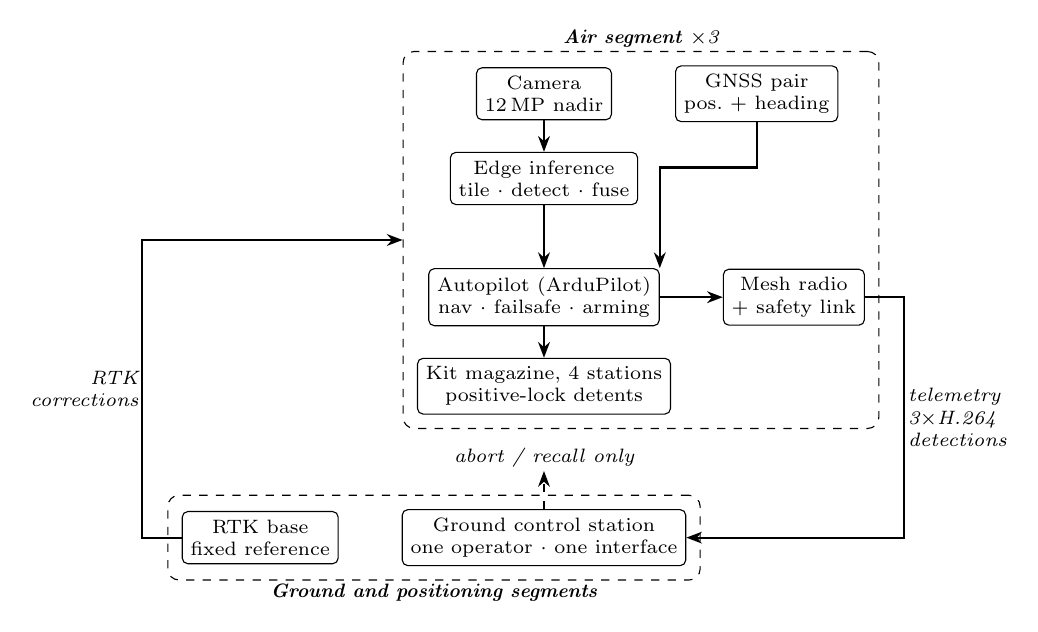
\begin{tikzpicture}[node distance=4mm]

% ---- air segment -----------------------------------------------------
\node[blk] (cam)  {Camera\\12\,MP nadir};
\node[blk, right=8mm of cam] (gnss) {GNSS pair\\pos.\ + heading};
\node[blk, below=4mm of cam] (inf) {Edge inference\\tile $\cdot$ detect $\cdot$ fuse};
\node[blk, below=8mm of inf] (fc) {Autopilot (ArduPilot)\\nav $\cdot$ failsafe $\cdot$ arming};
\node[blk, right=8mm of fc] (rad) {Mesh radio\\+ safety link};
\node[blk, below=4mm of fc] (mag) {Kit magazine, 4 stations\\positive-lock detents};

\draw[flow] (cam) -- (inf);
\draw[flow] (inf) -- (fc);
\draw[flow] (gnss) -- (gnss|-inf.north) -- ++(0,-2mm) -| (fc.north east);
\draw[flow] (fc) -- (mag);
\draw[flow] (fc) -- (rad);

\begin{scope}[on background layer]
\node[seg, fit=(cam)(gnss)(inf)(fc)(rad)(mag),
      label={[lbl]above:\textbf{Air segment} $\times$3}] (air) {};
\end{scope}

% ---- ground and positioning -----------------------------------------
\node[blk, below=12mm of mag] (gcs) {Ground control station\\one operator $\cdot$ one interface};
\node[blk, left=8mm of gcs] (rtk) {RTK base\\fixed reference};

\begin{scope}[on background layer]
\node[seg, fit=(gcs)(rtk),
      label={[lbl]below:\textbf{Ground and positioning segments}}] (gnd) {};
\end{scope}

\draw[flow] (rad.east) -- ++(5mm,0) |- (gcs.east)
      node[lbl, pos=0.25, right, align=left]
      {telemetry\\3$\times$H.264\\detections};
\draw[dflow] (gcs.north) -- (gcs.north|-gnd.north) -- ++(0,3mm)
      node[lbl, above, align=center] {abort / recall only};
\draw[flow] (rtk.west) -- ++(-5mm,0) |- (air.west)
      node[lbl, pos=0.25, left, align=right] {RTK\\corrections};

\end{tikzpicture}}
\caption{System architecture. The only permitted downlink commands are abort and
recall; the ground station is architecturally incapable of originating a retask,
waypoint change or drop command. Detection runs onboard, so the downlink serves
the operator rather than the algorithm.}
\label{fig:arch}
\end{figure}

\subsubsection{Air segment}
Three identical quadrotors, each carrying a Pixhawk-standard autopilot running
ArduPilot, a dual-band NavIC/GNSS receiver pair for position and moving-baseline
heading, a nadir-mounted 12\,MP camera, an edge inference module, a four-station
kit magazine with positive-lock detents, a mesh radio for telemetry and video,
and an independent sub-gigahertz safety link.

\subsubsection{Ground segment}
A single ground control station presenting one unified operator interface. The
station is architecturally incapable of originating a retask, waypoint change or
drop command; abort and recall are the only permitted downlink commands, and are
implemented as an explicit exception. This is a structural safety property rather
than a policy: the relevant code paths are absent from the deployed build, not
merely guarded.

\subsubsection{Positioning segment}
A team-owned RTK base station, positioned and set to a fixed reference from its
first three-dimensional fix within the setup window. Launch is gated on a
three-dimensional fix rather than an RTK fix; the first geotag is gated on
RTK-fixed, and detections made before convergence are geotagged in float and
re-fused once fixed. This decoupling recovers approximately ninety seconds of
setup time that a survey-in procedure would otherwise consume.

\subsection{Geolocation error budget}
\label{sec:geotag}

Survivor coordinate accuracy is the primary system output, and the error budget
is therefore the governing analysis of the whole design. Total error is the root
sum of squares of GNSS position error, boresight and lever-arm residual, attitude
error, terrain-model error and timing skew.

Table~\ref{tab:geotag} shows the dominant conclusion: positioning quality, not
optics, governs. This is what makes RTK a scoring requirement rather than an
optimisation, and it is why the two GNSS receivers survive every cost-reduction
pass in Section~\ref{sec:budget}.

\begin{table}[t]
\caption{Geolocation error by configuration}
\label{tab:geotag}
\centering
\small
\begin{tabular}{@{}llr@{}}
\toprule
\textbf{Case} & \textbf{Configuration} & \textbf{RSS error} \\
\midrule
A & No RTK, single-frame            & 3.09\,m \\
B & RTK, single-frame               & $\sim$1.3\,m \\
C & RTK + multi-frame fusion +      & \textbf{0.91\,m} \\
  & calibrated ground plane         & \\
\bottomrule
\end{tabular}
\end{table}

Multi-frame fusion is effectively free. At 60\,m altitude and 8\,m/s
groundspeed, forward overlap yields on the order of fourteen independent
observations of each target per pass even at a conservative 2\,Hz inference
rate. Those observations are used both for temporal confirmation, which
suppresses false positives, and for geolocation averaging.

\subsection{Perception and inference budget}

A 12\,MP sensor at 60\,m yields a ground sample distance of approximately
2\,cm/px, at which a supine adult subtends roughly fifty pixels --- small, but
within reach of tiled inference. Running detection on the full-resolution frame
would require 48 tiles per frame and is far beyond the thermal and compute
envelope of any module in this mass class. A two-times downsample with 20\,\%
tile overlap requires 12 tiles per frame; at a 2\,Hz inference rate this is 24
inferences per second at $640\times640$, which is within the demonstrated
throughput of a 20-TOPS-class edge module.

This is the single most benchmark-sensitive figure in the design. Published
throughput for comparable models on comparable hardware spans roughly 24 to 41
frames per second, and the lower end of that range leaves no margin. Hardware
benchmarking before design freeze is accordingly a funded, scheduled activity
rather than an assumption.

\subsection{Communications}

Regulatory rules require the ground station to display a live camera feed from
\emph{each} aircraft. Three independent MJPEG streams would demand 4.5--6\,Mbps
against a link budget of approximately 2.5\,Mbps. The system therefore uses
H.264 encoding served through a media gateway, carrying three concurrent
WebRTC streams in approximately 2.7\,Mbps, with per-feed rate reduction under
congestion rather than feed switching. Detection runs onboard; the downlink
serves the operator, not the algorithm.

An independent sub-gigahertz link in the 865--867\,MHz Indian delicensed
short-range-device band provides a command and safety path that does not share a
failure mode with the primary mesh.

\subsection{Payload delivery}

Kits are released at 6\,m above ground level, gated on a residual groundspeed
below 0.3\,m/s. At that release state, ballistic dispersion contributes
approximately 0.32\,m to total delivery error; combined with geolocation and
position-hold error the root-sum-square is approximately 1.5\,m with RTK
active. Release altitude is chosen low enough that wind drift remains under a
metre in realistic conditions, and high enough for safe clearance above a person
and above debris.

Positive-lock mechanical detents on each station ensure that a power interruption
cannot release a kit. This is treated as a safety-critical item and is excluded
from cost reduction by policy.

\subsection{Mission sequence}

Fig.~\ref{fig:flow} shows the autonomous mission sequence. Two properties are
worth drawing out. First, the launch stagger lives in the mission file as an
explicit delay before each take-off command, not in operator timing --- this is
what converts a 1.31\,m closest approach into the 64.80\,m of
Fig.~\ref{fig:launch}. Second, every terminal branch converges on
return-to-launch: link loss, low battery and operator abort share one recovery
path rather than three.

\begin{figure}[t]
\centering
\resizebox{0.86\columnwidth}{!}{%
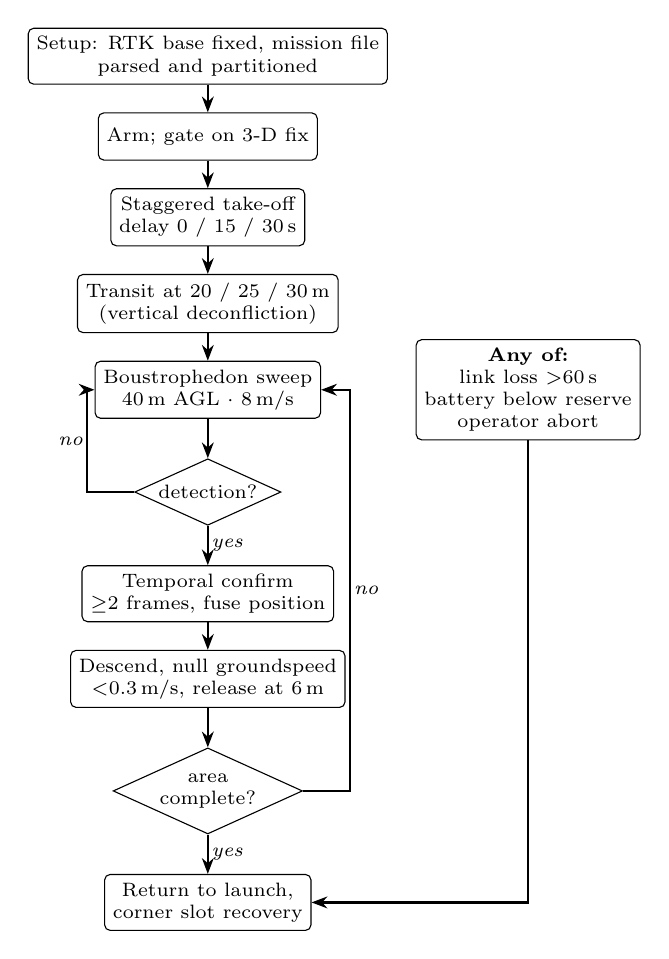
\begin{tikzpicture}[node distance=3.5mm]

\node[blk] (setup) {Setup: RTK base fixed, mission file\\parsed and partitioned};
\node[blk, below=of setup] (arm) {Arm; gate on 3-D fix};
\node[blk, below=of arm] (to) {Staggered take-off\\delay 0 / 15 / 30\,s};
\node[blk, below=of to] (tr) {Transit at 20 / 25 / 30\,m\\(vertical deconfliction)};
\node[blk, below=of tr] (sw) {Boustrophedon sweep\\40\,m AGL $\cdot$ 8\,m/s};
\node[dec, below=5mm of sw] (det) {detection?};
\node[blk, below=5mm of det] (conf) {Temporal confirm\\$\geq$2 frames, fuse position};
\node[blk, below=of conf] (del) {Descend, null groundspeed\\$<$0.3\,m/s, release at 6\,m};
\node[dec, below=5mm of del] (more) {area\\complete?};
\node[blk, below=5mm of more] (rtl) {Return to launch,\\corner slot recovery};

\node[blk, right=12mm of sw, align=center] (fail)
  {\textbf{Any of:}\\link loss $>$60\,s\\battery below reserve\\operator abort};

\draw[flow] (setup)--(arm);
\draw[flow] (arm)--(to);
\draw[flow] (to)--(tr);
\draw[flow] (tr)--(sw);
\draw[flow] (sw)--(det);
\draw[flow] (det)--(conf) node[lbl,pos=0.5,right]{yes};
\draw[flow] (conf)--(del);
\draw[flow] (del)--(more);
\draw[flow] (more)--(rtl) node[lbl,pos=0.5,right]{yes};
\draw[flow] (det.west) -- ++(-6mm,0) |- (sw.west) node[lbl,pos=0.25,left]{no};
\draw[flow] (more.east) -- ++(6mm,0) |- (sw.east) node[lbl,pos=0.25,right]{no};
\draw[flow] (fail.south) |- (rtl.east);

\end{tikzpicture}}
\caption{Autonomous mission sequence. The take-off stagger is encoded in the
mission file rather than in operator timing, and all three abnormal conditions
converge on a single return-to-launch path.}
\label{fig:flow}
\end{figure}

%=============================================================================
\section{Methodology and Work Plan}
%=============================================================================

The programme is organised into ten phases. Phases P1--P5 are analysis,
procurement and integration; P6--P10 are progressively more demanding flight
test. The eight-week flight-test window spanned by P6--P10 is the binding
schedule constraint on the entire programme, and the work plan is arranged to
protect it.

\begin{table}[t]
\caption{Programme phases}
\label{tab:phases}
\centering
\small
\begin{tabular}{@{}cp{2.05cm}p{4.3cm}@{}}
\toprule
\textbf{Ph.} & \textbf{Title} & \textbf{Principal exit criterion} \\
\midrule
P1  & Requirements and sizing & Design point frozen; all models regenerate \\
P2  & Ground segment          & Single-operator interface demonstrated against three simulated aircraft \\
P3  & Autonomy               & Deterministic plan generation; deconfliction verified in simulation \\
P4  & Fault handling         & Link-loss and low-battery behaviour verified by fault injection \\
P5  & Procurement and build  & Three airframes assembled and weighed; thrust stand complete \\
P6  & First flight           & Hover, trim, vibration and thermal characterisation \\
P7  & Perception field trials & Detection recall measured on real imagery with surveyed ground truth \\
P8  & Delivery trials        & Delivery CEP measured against a surveyed target mat \\
P9  & Full mission rehearsal & End-to-end mission with all three aircraft, no operator intervention \\
P10 & Setup and contingency  & Setup drill timed over repeated runs; margin recovered \\
\bottomrule
\end{tabular}
\end{table}

\subsection{Verification strategy}
\label{sec:evidence}

The programme's verification discipline is, we believe, its most transferable
contribution, and it exists because of a specific and recurring class of defect.

On four separate occasions during preparatory work, a configuration artefact was
found to be correct, unit-tested, reviewed, and \emph{not in the execution path}
of the running system. In one instance a validated failsafe parameter set was
never loaded by any simulation, so every test ran against stock defaults in which
the low-battery action was disabled. In another, a message-routing configuration
started cleanly and forwarded zero messages for weeks. Each of these reviewed
clean and had passing tests around it.

The countermeasure adopted is procedural rather than technical: no capability is
considered demonstrated until the real artefact has been exercised end to end and
the resulting values read back off the running system. Consequently every claim
in this proposal carries an explicit evidence class, and those classes are
maintained mechanically rather than editorially:

\begin{itemize}
  \item \textbf{Measured} --- observed on a running system, in software or in
        hardware-in-the-loop simulation.
  \item \textbf{Modelled} --- computed by a model whose inputs are themselves
        assumptions, and which regenerates in continuous integration.
  \item \textbf{Assumed} --- neither measured nor modelled; carried explicitly
        as a risk.
\end{itemize}

A continuous-integration job enforces the rule that every published number
regenerates byte-for-byte from its model, so that changing a model without
committing its regenerated output fails the build. Thirteen model outputs are
currently under this gate.

%=============================================================================
\section{Preliminary Results}
%=============================================================================

Substantial work has been completed before this request. We summarise it here
with the evidence class of each result stated, because a claim whose basis is
declared can be independently checked, whereas a claim whose basis is left
implicit cannot be.

\subsection{Measured in simulation}

\begin{itemize}
  \item \textbf{Low-battery failsafe returns the aircraft to the pad.}
        Verified across three simultaneous software-in-the-loop autopilots;
        return-to-launch triggered at 10\,809\,mAh of a 10\,800\,mAh planned
        consumption.
  \item \textbf{Three aircraft on one ground station.} A single telemetry
        router carried three distinct system identifiers to one ground station
        port with all three arriving.
  \item \textbf{Inter-aircraft separation at launch.} Staggered take-off delays
        encoded in the mission file, rather than in operator timing, increased
        the closest airborne approach during launch from 1.31\,m to
        \textbf{64.80\,m} (Fig.~\ref{fig:launch}). Both figures are recomputed
        directly from the committed telemetry.
  \item \textbf{Separation during the sweep.} Minimum airborne separation away
        from the pad is \textbf{29.19\,m}, with staggered transit altitudes of
        20/25/30\,m providing vertical deconfliction independent of the lateral
        plan.
  \item \textbf{Recovery deconfliction.} Assigning landing slots to the corners
        of the recovery pad rather than in a row increased slot spacing from
        1.22\,m to 2.61\,m at no cost, raising the measured minimum approach
        from an overlapping 0.83\,m to \textbf{2.27\,m} --- a clearance of
        1.22\,m between airframes (Fig.~\ref{fig:pad}). Separation while stacked
        in the air over the pad improves by the same mechanism.
  \item \textbf{Ground station.} All eight required operator displays were
        verified against three simultaneous autopilots, carrying three
        concurrent H.264 streams within the link budget, with offline map tiles
        (Fig.~\ref{fig:gcs}).
\end{itemize}

\begin{figure*}[t]
\centering
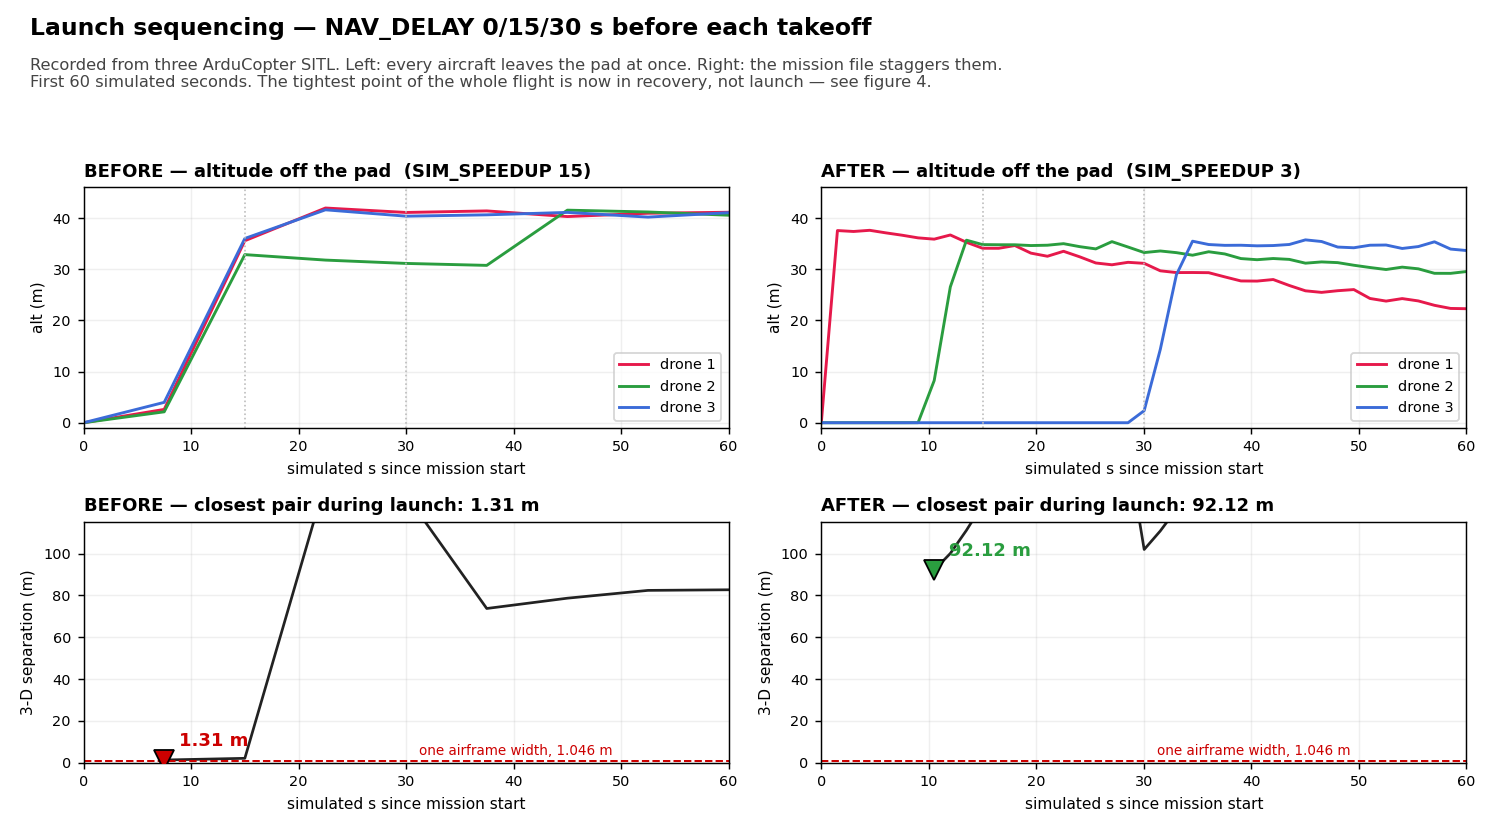
\includegraphics[width=\textwidth]{proof-1-launch.png}
\caption{Launch deconfliction, recorded from three ArduCopter software-in-the-loop
autopilots. Left: all three aircraft leave the pad together and the closest pair
passes within 1.31\,m --- inside one airframe width. Right: a delay encoded in
the mission file before each take-off command staggers them, and the closest
airborne pair is 64.80\,m. Both figures are reproducible from the committed
telemetry.}
\label{fig:launch}
\end{figure*}

\begin{figure}[t]
\centering
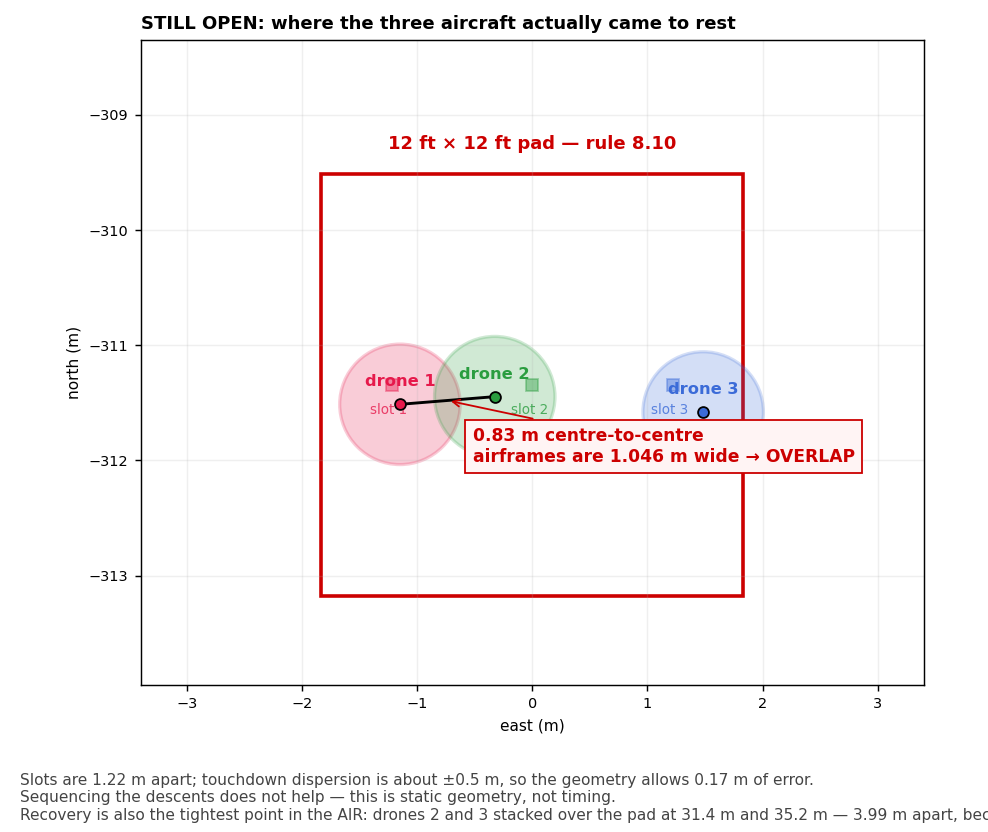
\includegraphics[width=\columnwidth]{proof-4-pad.png}
\caption{Recovery deconfliction on the landing pad. Slot centres must remain half
an airframe inside the pad edge, so they occupy a 2.61\,m square; a row across
that square gives 1.22\,m of spacing, its corners give the full 2.61\,m. The
measured closest approach at any time rises from an overlapping 0.83\,m to
2.27\,m --- twice the separation, same pad, no cost.}
\label{fig:pad}
\end{figure}

\begin{figure}[t]
\centering
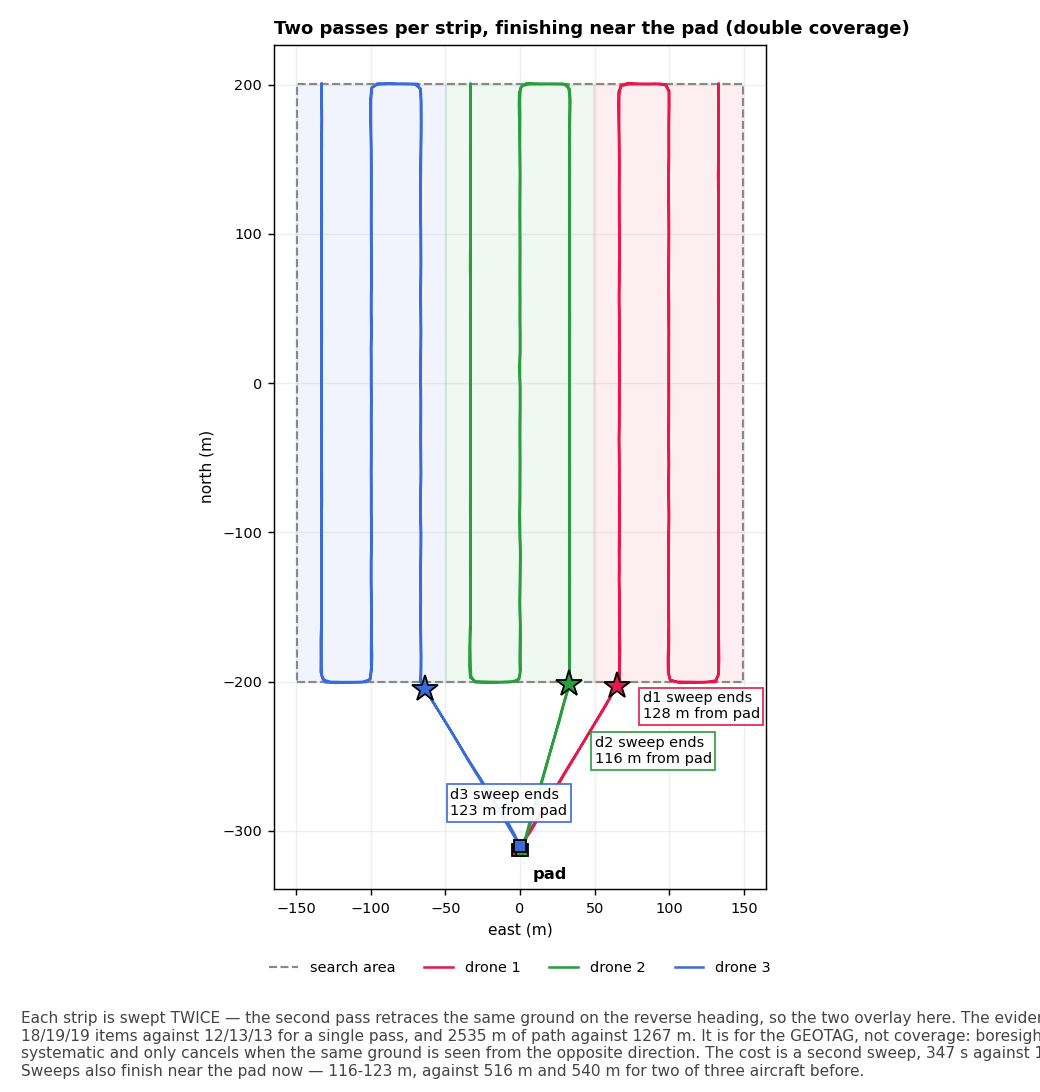
\includegraphics[width=\columnwidth]{proof-2-sweep.png}
\caption{Coverage decomposition and return geometry. Each aircraft is assigned an
equal-area strip and flies a boustrophedon pattern within it. Enumerating the
four start-side and direction combinations and keeping the one that ends nearest
home brings all three aircraft back within 116--128\,m of the pad, against
516\,m and 540\,m for two of three aircraft under the previous index-keyed rule
--- at identical path length.}
\label{fig:sweep}
\end{figure}

\begin{figure*}[t]
\centering
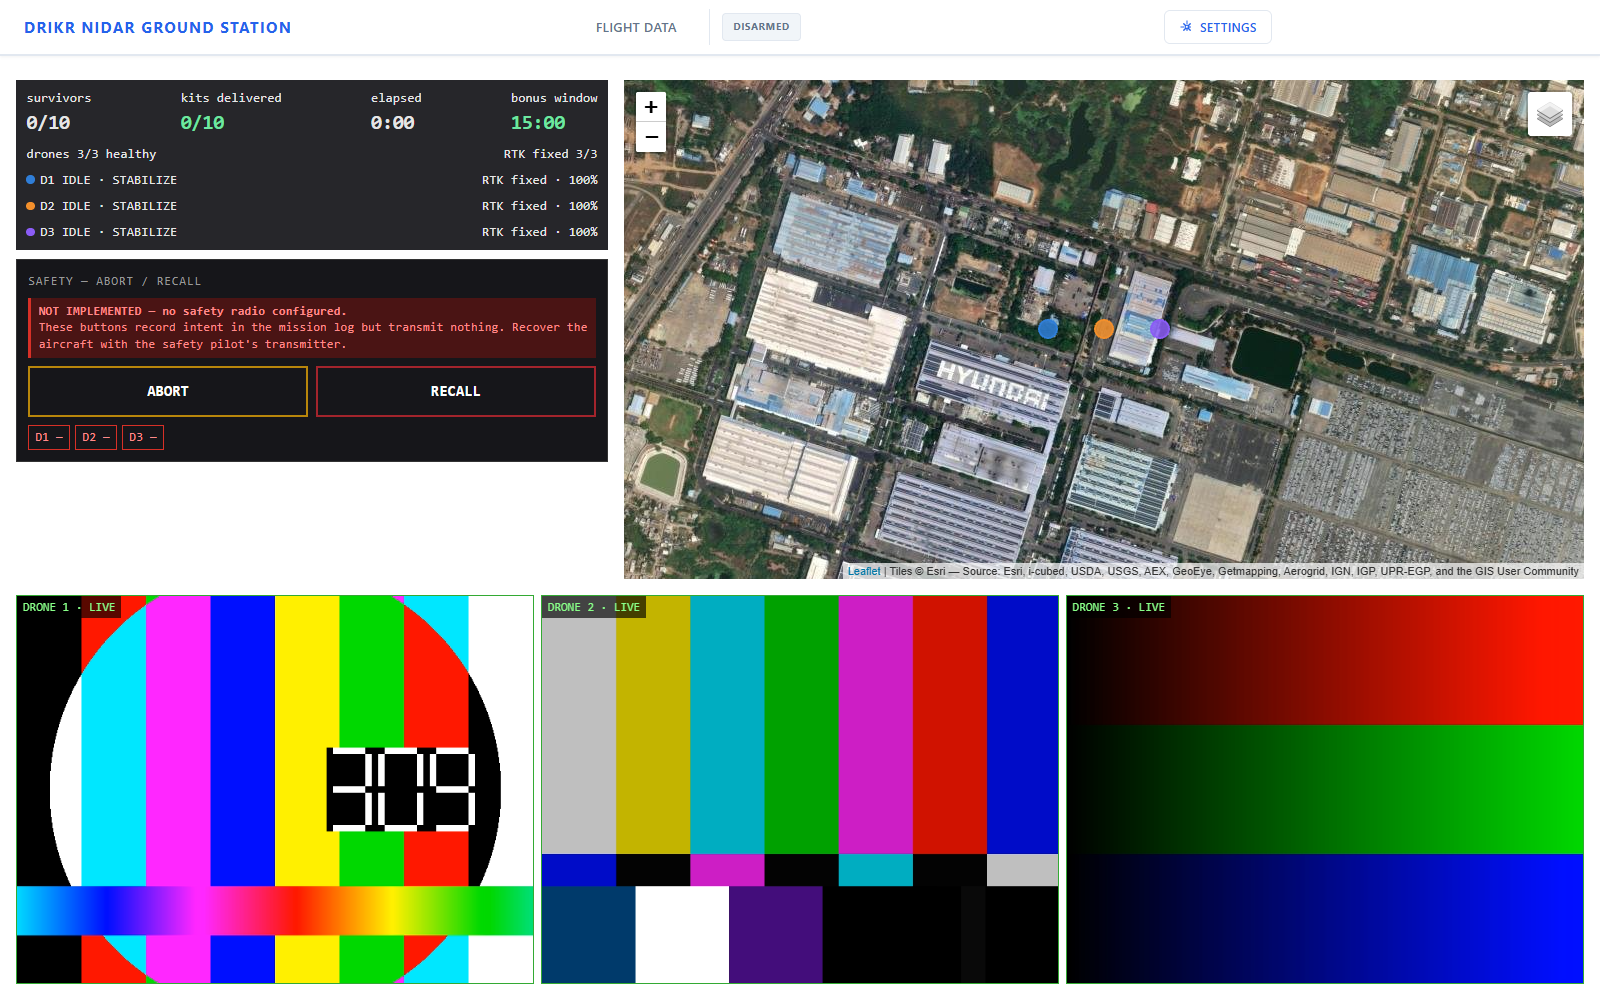
\includegraphics[width=0.92\textwidth]{gcs-running.png}
\caption{Ground control station carrying three concurrent H.264 streams within
the link budget, with offline map tiles and per-aircraft status. Note the
safety panel: abort and recall currently record operator intent in the mission
log but transmit nothing, because no safety radio is yet configured. This is
reported here rather than cropped out --- see Section~VI-C.}
\label{fig:gcs}
\end{figure*}

\subsection{Modelled}

Endurance, hover power, mass budget, thermal margin, link budget, delivery
dispersion and geolocation error are all modelled and regenerate from source.
The geolocation Monte Carlo reconciles with the independent analytic budget to
within one per cent, and the geotag projection has been verified
self-consistent between two independent formulations to $7.8\times10^{-10}$\,m.

\subsection{Assumed, or not yet implemented}

Detection recall on real post-flood imagery, boresight calibration residual,
achieved RTK accuracy in the field, and battery internal resistance under Indian
ambient conditions are all assumed. Each requires hardware and is a funded
activity in P5--P8.

One ground-segment function is explicitly \emph{not} implemented and is visible
as such in Fig.~\ref{fig:gcs}: the abort and recall controls currently record
operator intent in the mission log but transmit nothing, because no safety radio
is yet configured. Recovery today depends on the safety pilot's transmitter.
Closing this is a P4 activity and is gated on the sub-gigahertz link discussed
in Section~IV-E.

\subsection{The honest summary}

\emph{Nothing in this programme has flown.} Every ``measured'' result above was
measured in simulation or in software. That rules out whole classes of logical
and integration error and rules out none of the physical ones. The requested
funding exists principally to convert the modelled and assumed rows of this
section into measured ones.

%=============================================================================
\section{Budget and Cost Analysis}
\label{sec:budget}
%=============================================================================

\subsection{Basis of estimate}

The cost basis is arithmetic over a bill of materials in which each line carries
an exact manufacturer part number, an Indian supplier, and a source. Lines are
classified by price provenance: \emph{listed} where a dated Indian retail price
was obtained, and \emph{quote required} where no public price exists. We regard
the distinction as material. Four of the six largest lines in the aircraft ---
the autopilot, the motor, the cells and the camera --- have no public price and
require supplier quotation, and the cost basis carries that uncertainty
explicitly rather than concealing it in a rounded figure.

\subsection{Cost reduction study}

A structured cost-reduction study was performed against the verified bill of
materials, producing four costed configurations of the same aircraft plus one
reduced-capability alternative. Table~\ref{tab:options} summarises them.

\begin{table}[t]
\caption{Costed configuration options (per aircraft)}
\label{tab:options}
\centering
\small
\begin{tabular}{@{}clrp{2.5cm}@{}}
\toprule
\textbf{Opt.} & \textbf{Description} & \textbf{INR} & \textbf{Capability impact} \\
\midrule
A & As verified          & 2\,90\,546 & Baseline \\
B & \textbf{Recommended} & \textbf{2\,59\,001} & None \\
C & Low cost             & 2\,07\,295 & Loses heading reference \\
D & Floor                & 1\,29\,632 & Loses RTK and inference spec \\
E & Reduced platform     & 37\,309    & Cannot fly the mission \\
\bottomrule
\end{tabular}
\end{table}

Option~B is the recommended basis. It realises a saving of \inr{31\,545} per
aircraft --- \inr{94\,635} across the fleet --- without sacrificing any
capability on which the system is assessed. Its principal component is the
substitution of the edge inference module for a single-board computer with a
26-TOPS accelerator, which meets the throughput specification at materially lower
cost and is conditional on the benchmark described earlier.

Two findings from the study are worth reporting because they run counter to the
usual direction of such exercises. First, the bill of materials was found to be
\emph{at or below market} on its largest propulsion line: the carried price was
below the lowest listed price for any comparable part, indigenous or imported.
Second, the sub-gigahertz safety link was found to be materially under-priced;
the carried figure does not purchase a compliant radio for the Indian delicensed
band, and the line requires an increase of approximately \inr{11\,855}. Both
corrections are incorporated in the figures presented here.

Options~D and E are reported for completeness and are not proposed. Option~D
represents the arithmetic floor for an aircraft that can still fly the mission
and is presented as evidence of that floor rather than as a plan; it already
sacrifices RTK positioning and the inference specification. Option~E is a
reduced training platform that cannot carry the payload and is discussed in
Section~\ref{sec:mule}.

\subsection{Programme cost}

\begin{table}[t]
\caption{Programme cost breakdown}
\label{tab:programme}
\centering
\small
\begin{tabular}{@{}lr@{}}
\toprule
\textbf{Element} & \textbf{INR} \\
\midrule
Air vehicles (3)                      & 7.93\,L \\
Payload, ground segment, test equipment, & \\
\quad spares and software             & 11.02\,L \\
\midrule
Subtotal                              & 18.96\,L \\
Duty and freight, on imported residual & 1.34\,L \\
Goods and services tax                 & 3.65\,L \\
Contingency                            & 4.79\,L \\
\midrule
\textbf{Total requested}               & \textbf{28.74\,L} \\
\bottomrule
\end{tabular}
\end{table}

We state plainly that this is a development programme rather than a product
build. It carries calibration and test equipment, a full spares set including a
spare airframe structure, and a field data campaign that a production unit would
not. The marginal cost of an additional deployable system is substantially
lower than the programme total and is the appropriate figure for any discussion
of scaled procurement.

\subsection{A note on the training platform}
\label{sec:mule}

Option~E in Table~\ref{tab:options} is a \inr{37\,309} training airframe. It
fails eight system requirements and cannot fly the mission; it is emphatically
not a low-cost variant of the proposed system. Its value is different: the
programme's binding constraint is an eight-week flight-test window currently
budgeted entirely on aircraft that do not yet exist and cannot be risked once
they do. Two or three training airframes, at roughly the cost of one inference
module, would fly from the first week of that window and absorb ground-station
integration, radio-path validation, setup-drill timing, failsafe verification on
real hardware, and crash-and-rebuild practice. We identify this as the highest
return-on-investment discretionary item in the budget.

%=============================================================================
\section{Indigenisation Strategy}
%=============================================================================

Indigenous content is measured, not asserted. Every line in the bill of
materials carries a declared Indian value fraction, and the aggregate is
computed rather than estimated, which makes the claim auditable.

Value-weighted Indian content across the priced bill of materials is
approximately 68\,\%. We note for precision that weighting the same data by
programme spend --- in which the air vehicle counts three times --- yields
approximately 65\,\%, and we report both rather than the more flattering figure
alone.

\begin{table}[t]
\caption{Indigenisation status by subsystem}
\label{tab:indig}
\centering
\small
\begin{tabular}{@{}lp{4.4cm}@{}}
\toprule
\textbf{Subsystem} & \textbf{Status} \\
\midrule
Autopilot        & Indian, Pixhawk-standard, domestically manufactured \\
Propulsion       & Indian motors, ESCs and propellers with published thrust data \\
Airframe         & Indian composite fabrication \\
Cells            & Indian, BIS-certified 21700 NMC \\
Camera           & Indian embedded-vision supplier \\
GNSS             & Indian receiver with NavIC L1+L5 support \\
Co-processor     & Indian RISC-V development kit \\
Inference module & \textbf{No Indian equivalent exists at this class} \\
\bottomrule
\end{tabular}
\end{table}

The inference accelerator is the one genuinely irreducible import, and we
declare it plainly rather than obscuring it. Mitigation is confined to what is
honest: an Indian carrier board, Indian enclosure and thermal design, an Indian
camera, and a model trained on Indian field data. We regard an explicit gap
analysis as more credible than a uniformly confident claim, and we note that the
domestic RISC-V development kit carried on the aircraft is a genuine
demonstration of Indian silicon in flight, albeit in a monitoring role rather
than as an accelerator.

%=============================================================================
\section{Risk Register}
%=============================================================================

\begin{table}[t]
\caption{Principal risks and mitigations}
\label{tab:risk}
\centering
\small
\begin{tabular}{@{}p{2.3cm}cp{3.6cm}@{}}
\toprule
\textbf{Risk} & \textbf{Sev.} & \textbf{Mitigation} \\
\midrule
Detection recall below target on real imagery
& High & Field data campaign funded in P7; tiling and fusion parameters tunable without hardware change \\
\addlinespace
Inference throughput below 2\,Hz on selected hardware
& High & Benchmark before design freeze; fallback to reduced tile count on a centre crop \\
\addlinespace
RTK capability unconfirmed on selected receiver
& High & Supplier confirmation is a gating procurement action; degraded mode already specified and flagged to the operator \\
\addlinespace
Flight-test window compressed by procurement delay
& High & Domestic sourcing halves lead times; training airframes decouple integration from airframe availability \\
\addlinespace
Recovery parachute sizing and supply
& Medium & No domestic supplier identified; import lead time and correct mass rating are open procurement actions \\
\addlinespace
Setup time exceeds allowance
& Medium & Currently modelled, not measured; timed drills are the highest-priority early test \\
\addlinespace
Airframe loss during test
& Medium & Spares set sized for one rebuild; training airframes absorb early-campaign risk \\
\bottomrule
\end{tabular}
\end{table}

We draw particular attention to the setup-time risk. It is currently supported
by a model with a modest margin and no measurement, and it gates the entire
mission. Timed bench drills are scheduled as the earliest hardware activity in
the programme for precisely this reason.

%=============================================================================
\section{Expected Outcomes and Deliverables}
%=============================================================================

\begin{enumerate}
  \item Three flight-qualified aircraft with a documented, market-verified and
        predominantly indigenous bill of materials.
  \item A single-operator ground control station demonstrated end to end against
        real aircraft, with no network dependency.
  \item A measured detection recall figure on real imagery with surveyed ground
        truth, replacing the current assumption.
  \item A measured delivery circular error probable against a surveyed target,
        replacing the current model.
  \item A measured setup-to-launch time distribution over repeated drills.
  \item An open, reproducible evidence base in which every published figure
        regenerates from its model under continuous integration.
  \item A supply-chain report identifying, for each subsystem, the domestic
        capability that exists, the capability that does not, and what would be
        required to close the gap.
\end{enumerate}

The seventh deliverable may prove the most durable. The exercise of sourcing a
complete airframe domestically, at component granularity and with verified
prices, produced a map of Indian UAV supply-chain maturity that we have not seen
published elsewhere, including the specific and narrow point at which it
currently fails.

%=============================================================================
\section{Conclusion}
%=============================================================================

We propose an autonomous three-aircraft system that addresses the localisation
bottleneck in post-flood search and rescue, sourced as far as domestic industry
presently permits, and engineered under a verification discipline that
distinguishes what has been demonstrated from what has merely been designed.

The system's design point, error budgets and cost basis are established and
reproducible. Its coordination and failsafe behaviour have been demonstrated in
hardware-in-the-loop simulation across three simultaneous autopilots. What
remains is the part that requires funding: to build the aircraft, fly them, and
replace the modelled and assumed quantities in Section~\ref{sec:evidence} with
measured ones.

We are asking for \lakh{28.74} to do that, and we have tried throughout this
document to make every number in it checkable.

%=============================================================================
\section*{Acknowledgment}
%=============================================================================

% Commented out rather than left as printing placeholder text. Uncomment and
% complete before submission -- name faculty mentors, the department, and any
% supplier who provided evaluation hardware or engineering support.
%
% The authors thank ... for ... .

The author thanks the Department of Electronics and Communication Engineering,
Thapar Institute of Engineering and Technology, for institutional support.

% \balance  % optional final-page column balancing; requires the `balance` package

\begin{thebibliography}{00}

\bibitem{kapoutsis2017darp}
A.~C. Kapoutsis, S.~A. Chatzichristofis, and E.~B. Kosmatopoulos,
``DARP: Divide areas algorithm for optimal multi-robot coverage path planning,''
\emph{Journal of Intelligent \& Robotic Systems}, vol.~86, pp.~663--680, 2017.

\bibitem{choset2000coverage}
H.~Choset,
``Coverage of known spaces: the boustrophedon cellular decomposition,''
\emph{Autonomous Robots}, vol.~9, no.~3, pp.~247--253, 2000.

\bibitem{choi2009cbba}
H.-L. Choi, L.~Brunet, and J.~P. How,
``Consensus-based decentralized auctions for robust task allocation,''
\emph{IEEE Transactions on Robotics}, vol.~25, no.~4, pp.~912--926, 2009.

\bibitem{akyon2022sahi}
F.~C. Akyon, S.~O. Altinuc, and A.~Temizel,
``Slicing aided hyper inference and fine-tuning for small object detection,''
in \emph{Proc. IEEE International Conference on Image Processing (ICIP)}, 2022,
pp.~966--970.

\bibitem{sambolek2021sard}
S.~Sambolek and M.~Ivasic-Kos,
``Automatic person detection in search and rescue operations using deep CNN
detectors,''
\emph{IEEE Access}, vol.~9, pp.~37 905--37 922, 2021.

\bibitem{zhu2021visdrone}
P.~Zhu \emph{et al.},
``Detection and tracking meet drones challenge,''
\emph{IEEE Transactions on Pattern Analysis and Machine Intelligence}, vol.~44,
no.~11, pp.~7380--7399, 2021.

\bibitem{mathisen2020airdrop}
S.~H. Mathisen, K.~Gryte, S.~Gros, and T.~A. Johansen,
``Precision deep stall landing of fixed-wing UAVs using nonlinear model
predictive control,''
\emph{Journal of Intelligent \& Robotic Systems}, vol.~101, no.~24, 2021.

\bibitem{takasu2009rtklib}
T.~Takasu and A.~Yasuda,
``Development of the low-cost RTK-GPS receiver with an open source program
package RTKLIB,''
in \emph{Proc. International Symposium on GPS/GNSS}, 2009.

\end{thebibliography}

\end{document}
